% !TEXroot=main.tex
\section{SLAM}
{
	\subsection{Überblick}
	{
		SLAM (\textit{Simultaneous Localization and Mapping, dt.: Simultane Positionsbestimmung und Kartierung}) beschreibt den Prozess, in welchem eine Karte durch Messdaten erstellt wird, wobei der Roboter selbst auf der Karte verordnet wird.
		Im Fall des Turtlebot geschieht dies mithilfe der Messdaten des LiDAR-Sensors, welcher die Entfernung von Objekten durch Laserstrahlen misst (\textit{siehe LiDAR-Sensor})	
	}

	\subsection{Positionierung}
	{
		Der Roboter wird anfangs auf den Mittelpunkt der, zu Beginn noch nicht vorhandenen Karte, welche erst durch Messdaten entsteht, platziert. Die Position des Roboters wird entsprechend der Bewegung seiner Motoren kalkuliert. Mithilfe des Umfangs der Reifen kann die bewegte Distanz errechnet werden, da dem Roboter die Winkeländerung der Motoren, z.B. eine Drehung dieser um 180°, bekannt ist. Diese werden an die Motoren übermittelt, wobei die Information noch an andere Teile weitergeleitet werden kann, hier der Microchip auf der Hauptplatine des Raspberry Pi 3 in der Mitte der Roboters, welcher damit Rechnungen, eben zur Positionskorrektur durchführen kann. Vereinfacht gilt daher bei einer geraden Bewegung
		\begin{equation}
			D = R \cdot U
		\end{equation} 
		
		Hierbei steht $D$ für die zurückgelegte Distanz, $R$ für die Umdrehungen der Motoren und $U$ für den Umfang der Reifen. Die Rotation, also die Drehung des Roboters, wird aus der Rotationsdifferenz beider Motoren berechnet. Dreht sich der rechte Motor weiter (größerer Winkel), so dreht sich der Roboter nach links, für eine Rechtsdrehung gilt das Gegenteil.
		Auf diese Weise kann nur aus den Daten, welche an der Motoren gesendet wird, errechnet werden wie weit und in welche Richtung der Roboter sich bewegt hat.
		Die benötigten Daten werden aus Odometrie-Daten gelesen. Dies sind interne Daten des Roboters, welche durch Messungen oder (wie oben genannt) Rechnungen erhält. Diese weichen durch Umwelteinflüsse und Messungenauigkeiten leicht von der Realität ab.
		
		
	}

	\subsection{Kartierung}
	{
		Die Kartierung erfolgt mithilfe der durch den LiDAR-Sensor gemessenen Daten. Dieser misst den Abstand des Roboters in verschiedene Richtungen punktartig. \newline  
		\begin{figure}[H]
			\begin{minipage}{0.5\textwidth}
				\centering
				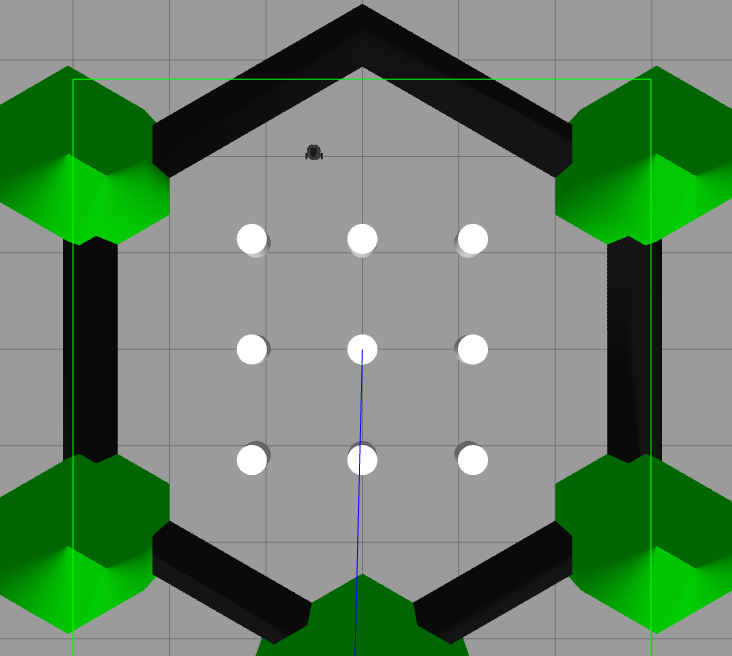
\includegraphics[height=5cm]{Bilder/virtualmap_world_gazebo.png}
				\caption{Roboter (zentriert im oberen \\ Drittel) in einer virtuellen \\Umgebung} %\parencite{flora85}}
				\label{pic:virtworldgazebo}
			\end{minipage}
			\begin{minipage}{0.5\textwidth}
				\centering
				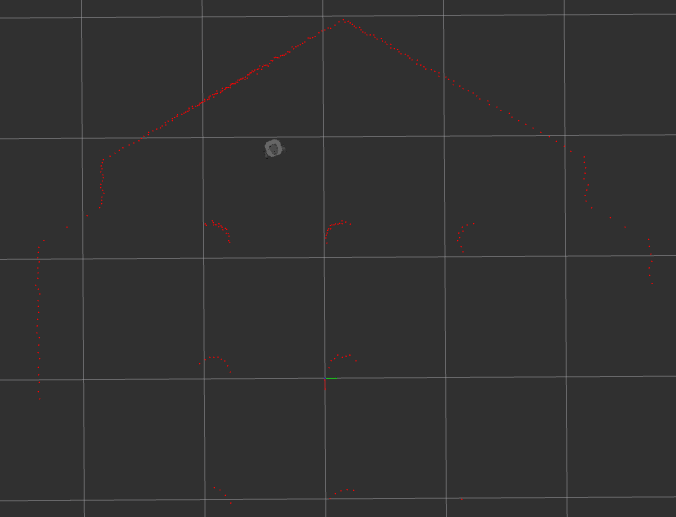
\includegraphics[height=5cm]{Bilder/virtualmap_world_rviz.png}
				\caption{Momentaufnahme der des LiDAR-Sensors gemessenen Punkte (Rot)}
				\label{pic:virtworldlaserrviz}	
			\end{minipage}
		\end{figure}
	
		Links erkennt man eine mit Gazebo simulierte Welt, in welcher sich der Roboter befindet, wobei er von Objekten (Säulen, Mauern) umgeben ist. Das rechte Bild ist ein Ausschnitt aus dem vorher erwähnte Programm Rviz, welches die durch den LiDAR-Sensor gemessene Punkte rot darstellt. Es ist zu erkennen, dass das Verbinden der Roten Punkte auf die Ursprüngliche Umgebung schließen lässt. Je näher der Roboter an einem Objekt ist, desto mehr Punkte befinden sich an dessen Stelle
		
		Zwar gibt eine Messung von einem Standpunkt einen akzeptablen Überblick, so werden jedoch viele Messungen von verschiedenen Stellen benötigt. Durch die Positionsänderung (\textit{siehe Positionierung}) kann errechnet werden wo neue Messpunkte im Vergleich zu alten Messpunkten liegen. Diese Positionierung der Punkte relativ zueinander wird schlussendlich zu einer Karte, wobei viele Messungen nötig sind. Da die Karte jedoch nur aus Punkten besteht, muss der Roboter diese noch interpretieren, sodass viele linear angeordnete Punkte z.B. als Wand interpretiert werden.
		
		Um eine komplette Karte zu erhalten Bewegt sich der Roboter durch die ihm noch unbekannte Welt, bis er eine Region durch genug Messpunkte Kartographiert hat und sich nun in Richtung einer ihm unbekannteren Region bewegen kann. Da der Roboter durch den LiDAR-Sensor konstant seine Umgebung misst, kann die Karte konstant verändert werden, vor allem, wenn der Roboter sich in Richtung weniger erforschte Gebiete bewegt.
		
		Während des Anfangs des Projektes wurde der Roboter noch mit Hilfe der Tastatur an einem Rechner oder über einen Logitech-Controller Gesteuert. Danach wurde daraus jedoch eine autonome Navigation, meist in Richtung von Gebieten, welche weniger erforscht sind. 
		
		Die Kartierung erfolgt mit Hilfe des \textit{gmapping}-Algorithmus. Dieser schaut sich die gescannten Laserdaten der \textit{sensor\textunderscore msgs/LaserScan}-Topic an und veröffentlicht drei Datenarten.
		\begin{enumerate}
			\item ein "Occupancy-Grid": 2D-Karte. Jeder Ort (Pixel) hat einen Ja/Nein Wert, welcher beschreibt, ob sich an der Position ein Objekt befindet oder nicht
			\item Entropie (Sicherheit über die Erkenntnis verschiedener Punkte: unsichere Punkte werden wahrscheinlicher geändert)
			\item Metadaten über die Karte.
		\end{enumerate}
	
		Durch die Kartierung dieses Algorithmus wird aus den einzelnen Laserscan-Daten nun eine Karte. Dies wird in den unteren Abbildungen dargestellt. Hierbei handelt es sich um die Karterung der in Abbildung 4 gezeigten Umgebung. Schwarze Punkte wurden als Hindernis erkannt, graue Stellen sind hindernisfreie Punkte. Die durch den LiDAR-Sensor gemessenen Punkte werden in grüner Farbe über die Karte gelegt. In Abbildung 7 und 8 ist zu erkenne, dass SChwarze Punkte nicht direkt mit Gemessenen Punkten des Lasers (grün) übereinstimmen. Dies liegt zum einen darin, dass die Berechnung der Karte Zeit benötigt, weshalb die Punkte noch verarbeitet werden, sowie daran, dass die Aktualisierungsrate der Karte eingestellt werden kann. Während intuitiv eine schnelle Aktualisierungsrate sinnvoll wirkt, ist eine zu schnelle Rate nachteilig, da viel Leistung benötigt wird und mehr Fehler gemacht werden, da ungenaue Messpunkte zu schnellen Schlüssen auf der Karte führen. Bei einer längeren Zeitdauer zwischen Kartenaktualisierungen können nämlich mehr gemessene Punkte in Betracht gemessen werden.
		
		\begin{figure}[H]
			\begin{minipage}{0.5\textwidth}
				\centering
				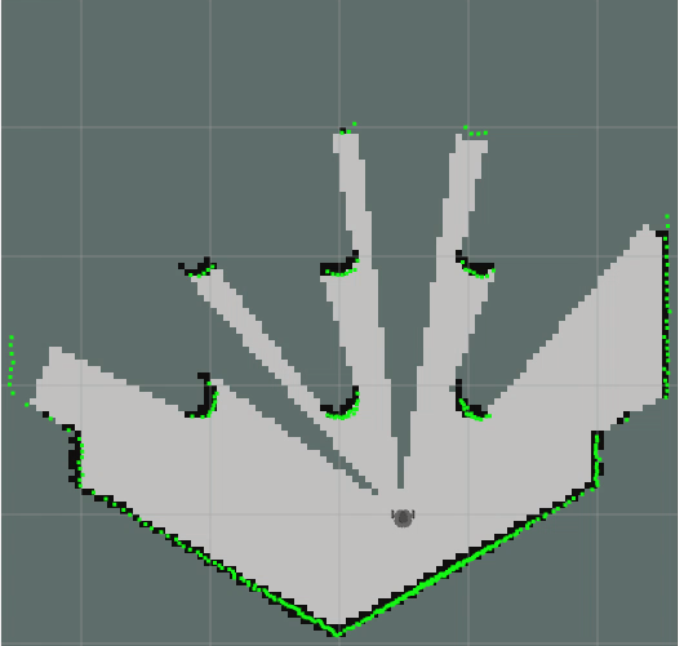
\includegraphics[height=5cm]{Bilder/mapping_smpl_1.png}
				\caption{Kartierung am Anfangspunkt}
				\label{pic:mapping_smpl_1}
			\end{minipage}
			\begin{minipage}{0.5\textwidth}
				\centering
				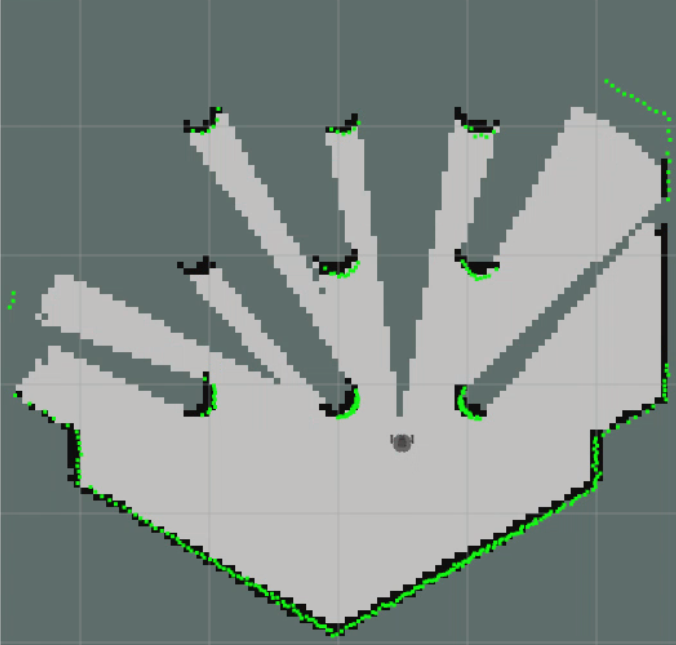
\includegraphics[height=5cm]{Bilder/mapping_smpl_2.png}
				\caption{Kartierung nach erster Bewegung (nach oben)}
				\label{pic:mapping_smpl_2}	
			\end{minipage}
		\end{figure}
		\begin{figure}[H]
			\begin{minipage}{0.5\textwidth}
				\centering
				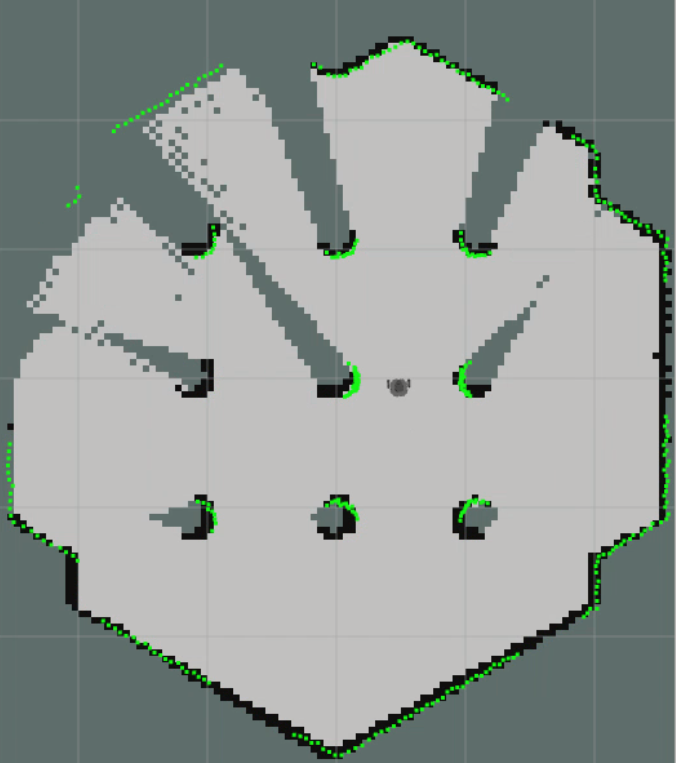
\includegraphics[height=5cm]{Bilder/mapping_smpl_3.png}
				\caption{Kartierung nach weiterer Bewegung}
				\label{pic:mapping_smpl_3}
			\end{minipage}
			\begin{minipage}{0.5\textwidth}
				\centering
				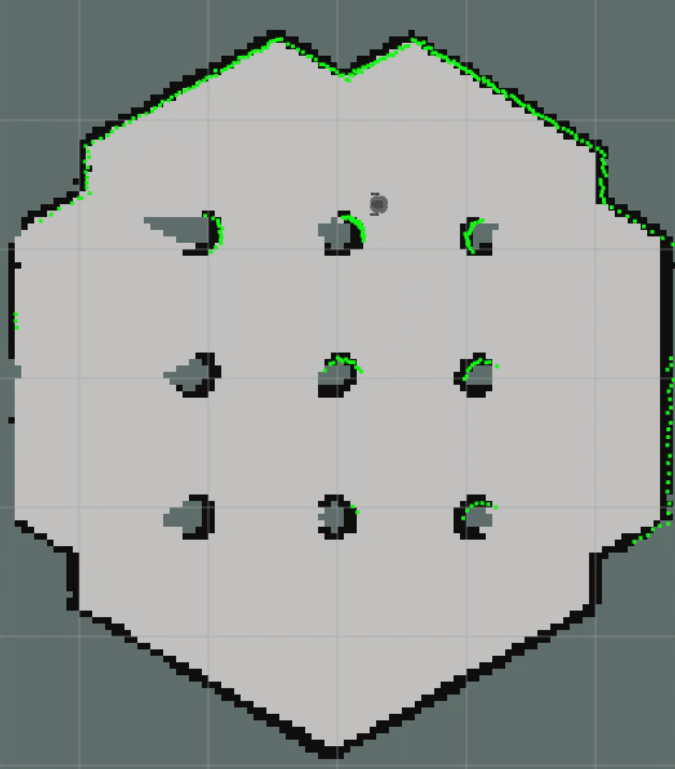
\includegraphics[height=5cm]{Bilder/mapping_smpl_4.png}
				\caption{Kartierung nach Erreichen des oberen Endes}
				\label{pic:mapping_smpl_4}	
			\end{minipage}
		\end{figure}
	}
}